% !TEX root = ./physics_of_fluids.tex
% !TEX TS-program = xelatex
% !TEX encoding = UTF-8 Unicode
\chapter{Boundary conditions and interfaces}
\label{chap:boundary_conditions}
We have seen in the previous chapter how to express mass and momentum conservation at the fluid particle level, and we have derived the corresponding equations for fluid motion. These equations are naturally associated with \textbf{boundary conditions} that either express conservation laws (e.g. no mass flux at a boundary) or peculiar physical processes occurring at a surface (temperature or velocity continuity). In both cases these boundary conditions will be pivoting in the determination of the solution.
\section{Fluxes at boundaries: impermeability and imbibition}
\begin{figure}[htbp]
\begin{center}
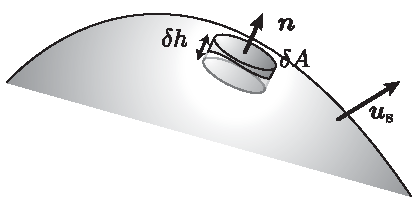
\includegraphics{impermeability.pdf}
\caption{Balance over an elementary volume located across a solid boundary.}
\label{fig:impermeability}
\end{center}
\end{figure}

Let's consider a solid moving in a fluid at velocity $\bu_\text s$ (possibly time dependent) and let's conduct a mass balance on a small cylindrical volume of base $\delA$ and height $\delh$ located across the fluid and the solid (Fig.~\ref{fig:impermeability}). Now let $\delh$ tends to 0 so that the mass element shrinks down to zero.  From now on, the mass variation of the element should necessarily be zero, and this implies that the mass flux from the fluid has to be balanced by the mass flux from the solid side:
\begin{equation}
-\lp\bj_\text{fluid}\cdot \bn_\text{fluid}\rp \delA -  \lp\bj_\text{solid}\cdot \bn_\text{solid}\rp \delA = 0.
\end{equation}
Let's write arbitrarily $\bn = \bn_\text{fluid} = - \bn_\text{solid}$ so that:
\begin{equation}
-\bj_\text{fluid}\cdot \bn +  \bj_\text{solid}\cdot \bn = 0.
\end{equation}
Without mixing phenomena, the fluid velocity $\bu$ already takes into account diffusive effects (it is the chemical species velocity) and the mass flux reduces to the convective flux. Beware that as we are in the solid reference frame, the relative velocity of the fluid is $\bu - \bu_\text s$, so that the mass flux on the fluid side is:
\begin{equation}
\bj_\text{fluid} = \rho \lp\bu-\bu_\text s\rp.
\end{equation}
\prg{The impermeable wall.\index{impermeability}} A very common case is that of an \textbf{imperméable} solid in which the fluid cannot penetrate; the fluid mass flux within the solid is therefore zero and $\bj_\text{solid} = \boldsymbol 0$. Mass conservation expressed at an impermeable boundary therefore reduces to:
\begin{equation}
\bu\cdot\bn = \bu_\text s \cdot\bn
\label{eq:impermeability}
\end{equation}
This is the \textbf{impermeability condition} for an object (or a wall). As the name implies, it simply expresses the fact that the fluid cannot penetrate into the solid. This condition takes the form of a \textbf{continuity of normal velocities}.
%
%Note : dans le cas particulier (mais très courant !) d'une objet solide fixe, cette condition devient  $\bu\cdot\bn =0$.
%\prg{Paroi perméable.} La discussion précédente s'étend naturellement au cas des parois perméables. Celles-ci peuvent correspondre à des tissus biologiques perméables à certains solutés, à des matériaux pouvant être imbibés par des solvants, des terrains trempés par la pluie ou encore des profils portants percés à des fins de contrôle de couche limite (comme la turbovoile de Cousteau et Malavard illustrée dans la séquence vidéo du cours).
%
%Le flux de masse au sein de la paroi n'est désormais plus nul et sa détermination requiert de connaître le type d'écoulement au sein du solide. Supposons toutefois la vitesse d'imbibition $\bu_\text{imbib}$ constante et connue (correspondant par exemple au cas d'une aspiration à débit imposé). La conservation de la masse à une paroi perméable mobile s'écrira alors :
%\begin{equation}
%\rho (\bu-\bu_\text s) \cdot \bn = \rho (\bu_\text{imbib}) \cdot \bn,
%\end{equation}
%soit 
%\begin{equation}
%\bu\cdot\bn = \lp\bu_\text s + \bu_\text{imbib}\rp\cdot\bn.
%\end{equation}
%\prg{Condition limite sur un champ de concentration à une paroi.}
%Les conditions limites à appliquer sur l'équation de transport d'un champ de concentration~(\ref{eq:conv_diff}) peuvent être obtenues suivant le même principe. Imaginons pour cela un champ de concentration transporté par un écoulement $\bu$ au sein duquel un solide (imperméable) se meut à la vitesse $\bu_\text s$. Dans le référentiel du solide le flux de matière à travers une surface $\delA \,\bn$ quelconque est :
%\begin{equation}
%\bj_\text{matière} = \bj_\text{conv} + \bj_\text{diff} = c \lp \bu - \bu_s\rp - D \nabla c.
%\end{equation}
%La condition d'imperméabilité de la paroi au champ de concentration $c$ s'écrit donc :
%\begin{equation}
%c (\bu-\bu_\text s) \cdot \bn - D \nabla c \cdot \bn = 0,
%\end{equation}
%car le flux de matière est nul dans le solide.
%En utilisant la condition d'imperméabilité du champ de vitesse~(\ref{eq:impermeabilite}), cette relation se réduit à :
%\begin{equation}
%\nabla c \cdot \bn \equiv \pd{c}{n} = 0.
%\end{equation}
%\prg{Transfert de masse à une interface : évaporation.} Un dernier exemple d'obtention de conditions limites à partir d'une équation de bilan est la condition de continuité du flux de masse à travers une interface liquide-gaz, dans le cas où le liquide s'évapore. 
%
%Effectuons un bilan de masse sur le même type d'élément de volume que celui considéré précédemment : un petit élément cylindrique de base $\delA$ et de hauteur $\delh$ à cheval sur l'interface se déplaçant à $\bu_\text i$. On fait tendre la hauteur $\delh$ de l'élément vers 0, de sorte à ce que la masse de l'élément tende vers 0 également. Le bilan de masse sur cet élément s'écrit :
%\begin{equation}
%\bj_\text{conv. liquide} = \bj_\text{conv. gaz} + \bj_\text{diff. gaz}
%\end{equation}
%soit :
%\begin{equation}
%\rho_\ell \lp\bu_\ell - \bu_\text i\rp \cdot \bn = \rho_v \lp\bu_g -\bu_\text i\rp\cdot \bn - D \nabla \rho_v \cdot n
%\end{equation}
%Si l'évaporation est très violente (e.g. front de combustion), le flux est dominé par les effets de convection et 
%$$\bu_g \sim \underbrace{\frac{\rho_\ell}{\rho_v}}_{\gg 1} \bu_\ell$$
%c'est-à-dire que l'écoulement (dit de Stefan) induit dans la vapeur est beaucoup plus violent que celui dans le liquide.
%Dans l'autre limite, où l'évaporation est très lente (cas d'une goutte d'eau séchant librement), c'est plutôt le terme diffusif qui domine.
%\section{Conditions phénoménologiques : adhérence aux parois et continuité}
%En plus des conditions précédentes découlant de principes de conservation, les fluides sont sujets à d'autres conditions limites, établies et confirmées sur des bases expérimentales et faisant l'objet d'un consensus, mais pas d'un démonstration exacte. Ces conditions phénoménologiques sont les conditions de \textbf{continuité des champs} aux interfaces, comme la vitesse, la température etc.
%
%\paragraph{$\rhd$ Une brève histoire de l'adhérence.} La condition d'adhérence, $\bu = \bu_\mathrm{s}$, a une histoire étonnante et pleine de rebondissements, dont nous traçons les grandes lignes dans ce qui suit \citep{Goldstein1950}. Au \textsc{XVIII}$^e$ siècle, la description théorique des écoulements potentiels (correspondant à l'approximation d'écoulement parfait de fluide) était déjà bien place, mais les comparaisons avec les expériences étaient médiocres. Daniel Bernoulli en était bien conscient et attribuait les différences entre les écoulements (parfaits) prédits et ceux observés expérimentalement à une ``condition d'adhérence'' qui devait prévaloir aux parois. Coulomb démontra par la suite expérimentalement qu'un disque oscillant dans un liquide ne semblait pas particulièrement affecté par un changement de ses propriétés de surface (lisse, rugueuse ou recouverte de graisse), si bien qu'il lui semblait également que la vitesse de l'écoulement correspondait à celle du disque. Dans cette vision, le fluide a les mêmes propriétés en tout point de l'espace, et il satisfait simplement une condition additionnelle à la paroi.
%
%Mais au cours du \textsc{XIX}$^e$ siècle des théories concurrentes sont apparues. Girard proposa ainsi que la couche liquide touchant la paroi avait des propriétés physiques différentes l'amenant à adhérer au solide. La couche directement adjacente (composée de fluide ``normal'') pouvait quant à elle glisser parfaitement sur la première. Navier s'intéressa également au problème et avança une condition limite impliquant un glissement proportionnel à la contrainte de cisaillement $\beta u = \mu \pd{u}{n}$, où le ratio $\mu/\beta$ a la dimension d'une longueur : la \textit{longueur de glissement}. Il s'en suivit une période de relative confusion, où les grands théoriciens de l'époque (Poisson, Stokes) ont adopté alternativement l'une ou l'autre des conditions limites.
%
%Au fil du temps cependant, des expériences fines conduites notamment par Couette ou Maxwell firent définitivement pencher la balance du côté de la condition d'adhérence. Maxwell suggéra sur des considérations moléculaires que si la condition de Navier est bien à l'\oe uvre, la longueur sur laquelle s'effectue le glissement est si petite -- de l'ordre de quelques libre-parcours moyens -- qu'il est très raisonnable de la considérer nulle, i.e. de considérer adhérence à la paroi : $\bu = \bu_\text s$. Ceci est en particulier respecté dans les conditions usuelles des expériences et laboratoires, mais pas nécessairement dans des conditions de gaz raréfiés (e.g. rentrée dans l'atmosphère, vol hypersonique) ou d'écoulements de longues chaînes de polymères (écoulements en piste microfluidique), comme le confirment les expériences.
%
%Au \textsc{XX}$^e$ siècle, l'accord quasiment parfait entre les observations expérimentales et la prédiction utilisant la condition d'adhérence pour de nombreux écoulements, comme l'écoulement de Poiseuille, de Couette, la chute de la sphère de Stokes en fluide visqueux, le seuil d'instabilité dans l'expérience de Taylor-Couette... ont définitivement convaincu de la validité de cette condition. 
%
%Par ailleurs, les lois d'échelle sur la traînée d'un objet déduites de l'analyse dimensionnelle sur la base des échelles caractéristiques $\rho, U, D$ et $\mu$ capturent l'évolution des efforts aérodynamiques sur une vaste plage d'échelles. Si une autre échelle de longueur (associée au glissement à la paroi) était pertinente dans la description des écoulements, les lois d'échelles s'en trouveraient modifiées. 
%
%On peut comprendre cette condition d'adhérence (continuité de $\bu$ de part et d'autre de l'interface) tout comme la condition de continuité des températures comme résultant d'équilibre à l'échelle moléculaire : les transferts extrêmement rapides entre molécules adjacentes induisent l'équilibrage instantané de la quantité de mouvement moyenne (vitesse) et de la vitesse d'agitation thermique (température) \citep{Batchelor1967}. À une interface entre un milieu I et un milieu II (solide-fluide, ou fluide-fluide), on aura donc :
%\begin{equation}
%\bu_\text I = \bu_\text{II} \quad \text{et} \quad T_\text I = T_\text{II}
%\end{equation}
